\chapter{Einleitung}
\label{cha:Einleitung}

\section{Motivation}
Für ERP-Softwarelösungen ist es wichtig möglichst auf die Wünsche des Kunden einzugehen. Dies beinhaltet auch die Anpassung an bereits existierende Konkurrenzlösungen. 
Um hier nicht für jeden Drittanbieter eine eigene Schnittstelle implementieren zu müssen, versucht man dies über eine Standardlösung, die international anerkannt ist, abzubilden. Hier hat sich speziell XML (eXtensible Markup Language) etabliert. Die genannten Schnittstellen müssen stetig adaptiert und angepasst werden. 

Dies führt zu einem großen Entwicklungsaufwand, was die Validierung der einzelnen Felder bei der Kommunikation betrifft. 
Im Vordergrund steht hier die Basisüberprüfung wie die Datentypen der einzelnen Felder. Weiteres sollen Pflicht- und Informationsfelder validiert werden, aber auch einfache Geschäftsregeln sollen kontrolliert werden können. 
Zum Beispiel gibt es verschiedene Befehle, die als Attribut von einzelnen XML-Elementen gesetzt werden. Aufgrund dieser Ausprägung müssen dann verschiedene andere Elemente mitgeliefert werden. Fehlen solche Abhängigkeiten, so ist die XML-Datei ungültig und soll nicht importiert werden.
Die so generierten Schemadateien sollen einerseits dem Fremdsystem zur Verfügung gestellt werden, als auch intern verwendet werden. 
Dem Fremdsystem soll es damit ermöglicht werden bereits von Inbetriebnahme der Schnittstelle beim Kunden, ihre Kommunikation mit BMD zu überprüfen. 

Hier bietet sich das XML Schema an, da dies ISO standardisiert ist und mit einer Vielzahl von Werkzeugen überprüft werden kann. 
Intern soll das XML Schema verwendet werden um Import-Dateien des Fremdsystem zu validieren und  um mögliche Fehlversuche zu verhindern. Deswegen wird das XML Schema auch intern generiert werden müssen, da die Schnittstelle jederzeit angepasst werden kann.
Da es oft eine Mehrzahl von Schnittstellen im Betrieb gibt, muss dies auch bei der Realisierung und Einbindung bedacht werden.


\section{Zielsetzung}
Das Ziel dieser Arbeit ist ein System, dessen Ausgabe eine XML-Schemadatei zur Validierung von XML-Dateien ist. Diese XML-Dateien dienen zum Austausch von Stamm- und Bewegungsdateien mit einem Fremdsystemen. Die definierten Schnittstellen zu den Fremdsystemen variieren hier sehr stark.
Als Basis der Überprüfung dient deswegen eine Auswahl von 
verschiedenen Feldern, wie in \ref{fig:Feldauswahl} dargestellt. Diese Felder repräsentieren jeweils 
eine Spalte einer relationalen Datenbank. Jede Auswahl ist 
wiederum in einer Tabelle gespeichert.Es müssen sowohl Oracle 
und Microsoft SQL Server unterstützt werden, da auch das ERP-System beide Datenbank-Systeme unterstützt. 
Konkret soll diese Software in das Modul der PPS (Produktionsplanungs- und Steuerungssystem) vom BMD Systemhaus GesmbH integriert werden. 
Dies bedeutet, dass das neue System keine eigenstehende Software sein soll/muss. 
Den Fremdsystemen werden nur die Schemadateien zur Verfügung gestellt.

\begin{figure}
    \centering
    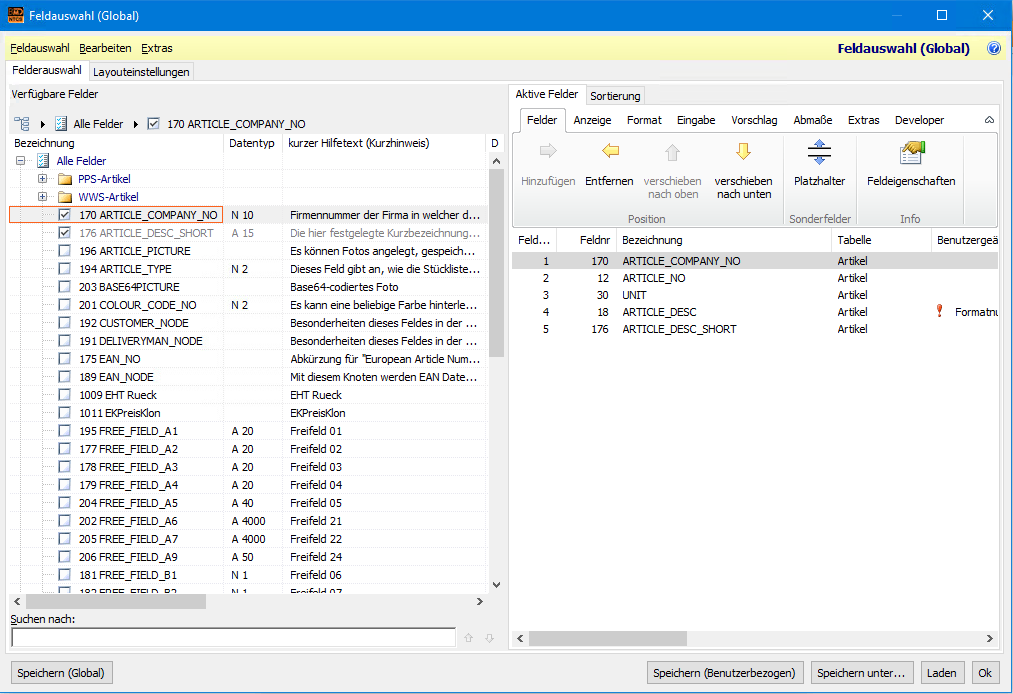
\includegraphics[width=.95\textwidth]{images/Feldauswahl.png}
    \caption{Definition Schnittstelle in BMD}
    \label{fig:Feldauswahl}
\end{figure}


% Dieses Dokument ist als vorwiegend technische Starthilfe für das
% Erstellen einer Masterarbeit (oder Bachelorarbeit) mit \latex
% gedacht und ist die Weiterentwicklung einer früheren
% Vorlage\footnote{Nicht mehr verfügbar.} für das Arbeiten mit
% Microsoft \emph{Word}. Während ursprünglich daran gedacht war, die
% bestehende Vorlage einfach in \latex zu übernehmen, wurde rasch
% klar, dass allein aufgrund der großen Unterschiede zum Arbeiten
% mit \emph{Word} ein gänzlich anderer Ansatz notwendig wurde. Dazu
% kamen zahlreiche Erfahrungen mit Diplomarbeiten in den
% nachfolgenden Jahren, die zu einigen zusätzlichen Hinweisen Anlass gaben.

% Das vorliegende Dokument dient einem zweifachen Zweck:
% \emph{erstens} als Erläuterung und Anleitung, \emph{zweitens} als
% direkter Ausgangspunkt für die eigene Arbeit. Angenommen wird,
% dass der Leser bereits über elementare Kenntnisse im Umgang mit
% \latex verfügt. In diesem Fall sollte -- eine einwandfreie
% Installation der Software vorausgesetzt -- der Arbeit nichts mehr
% im Wege stehen. Auch sonst ist der Start mit \latex\ nicht
% schwierig, da viele hilfreiche Informationen auf den zugehörigen
% Webseiten zu finden sind %%(s.\ Kap.~\ref{cha:ArbeitenMitLatex}).





% \section{Warum {\latex}?}

% Diplomarbeiten, Dissertationen und Bücher im
% technisch-natur\-wissen\-schaft\-lichen Bereich werden
% traditionell mithilfe des Textverarbeitungssystems \latex
% \cite{Lamport1994, Lamport1995} gesetzt. Das hat gute Gründe, denn
% \latex ist bzgl.\ der Qualität des Druckbilds, des Umgangs mit
% mathematischen Elementen, Literaturverzeichnissen etc.\
% unübertroffen und ist noch dazu frei verfügbar. Wer mit \latex
% bereits vertraut ist, sollte es auch für die Abschlussarbeit
% unbedingt in Betracht ziehen, aber auch für den Anfänger sollte
% sich die zusätzliche Mühe am Ende durchaus lohnen.

% Für den professionellen elektronischen Buchsatz wurde früher
% häufig \emph{Adobe Framemaker} verwendet, allerdings ist diese
% Software teuer und komplex. Eine modernere Alternative dazu ist
% \emph{Adobe InDesign}, wobei allerdings die Erstellung
% mathematischer Elemente und die Verwaltung von Literaturverweisen
% zur Zeit nur rudimentär unterstützt werden.
% \footnote{Angeblich werden aber für den (sehr sauberen) Schriftsatz 
% in \emph{InDesign} ähnliche Algorithmen wie in \latex\ verwendet.}

% Microsoft \emph{Word} gilt im Unterschied zu \latex, 
% \emph{Framemaker} und \emph{InDesign} übrigens nicht als professionelle
% Textverarbeitungssoftware, obwohl es immer häufiger auch von
% großen Verlagen verwendet wird.
% \footnote{Siehe auch \url{http://latex.tugraz.at/mythen.php}.}
% Das Schriftbild in \emph{Word}
% lässt -- zumindest für das geschulte Auge -- einiges zu wünschen
% übrig und das Erstellen von Büchern und ähnlich großen Dokumenten
% wird nur unzureichend unterstützt. Allerdings ist \emph{Word} sehr
% verbreitet, flexibel und vielen Benutzern zumindest oberflächlich
% vertraut, sodass das Erlernen eines speziellen Werkzeugs wie
% \latex\ ausschließlich für das Erstellen einer Abschlussarbeit
% manchen verständlicherweise zu mühevoll ist. Es sollte daher
% niemandem übel genommen werden, wenn er/sie sich auch bei der Abschlussarbeit
% auf \emph{Word} verlässt. Im Endeffekt lässt sich mit etwas
% Sorgfalt (und ein paar Tricks) auch damit ein durchaus akzeptables
% Ergebnis erzielen. 
% Ansonsten sollten auch für \emph{Word}-Benutzer 
% einige Teile dieses Dokuments von Interesse sein, insbesondere die
% Abschnitte über Abbildungen und Tabellen
% %%(Kap.~\ref{chap:Abbildungen}) und mathematische Elemente
% %%(Kap.~\ref{chap:Mathematik}).

% Übrigens, genau hier am Ende des Einleitungskapitels (und nicht
% etwa in der Kurzfassung) ist der richtige Platz, um die
% inhaltliche Gliederung der nachfolgenden Arbeit zu beschreiben.
% Hier soll dargestellt werden, welche Teile (Kapitel) der Arbeit
% welche Funktion haben und wie sie inhaltlich zusammenhängen. Auch
% die Inhalte des \emph{Anhangs} -- sofern vorgesehen -- sollten hier
% kurz beschrieben werden.
